\documentclass[twocolumn,superscriptaddress,aps]{revtex4-1}

\usepackage[utf8]{inputenc}

\usepackage{amsfonts}
\usepackage{amssymb}
\usepackage{amsmath}
\usepackage{amsthm}

\usepackage{bm}
\usepackage{cancel}
\usepackage{bbold}
\usepackage{bm}
\usepackage{slashed}
\usepackage{graphicx}
\usepackage{color}
\usepackage{hyperref}
\usepackage{algorithm}
\usepackage{algpseudocode}
\usepackage{tikz}

\newcommand{\glnote}[1]{\textcolor{red}{[GL: #1]}}
\newcommand{\kcnote}[1]{\textcolor{red}{[KC: #1]}}

\newcommand{\qxpsi}{q(\mathbf{x}|\bfpsi)}
\newcommand{\bftheta}{{\bm \theta}}
\newcommand{\bfpsi}{{\bm \psi}}
\newcommand{\bfx}{\mathbf{x}}
\newcommand{\bfz}{\mathbf{z}}

\theoremstyle{plain}
\newtheorem{theorem}{Theorem}
\newtheorem{proposition}[theorem]{Proposition}

\begin{document}


% ==============================================================================

\title{\Large{Adversarial Variational Optimization of Non-Differentiable Simulators}}
\vspace{1cm}
\author{\small{\bf Gilles Louppe}\thanks{\texttt{g.louppe@nyu.edu}}}
\affiliation{New York University}
\author{\small{\bf Kyle Cranmer}\thanks{\texttt{kyle.cranmer@nyu.edu}}}
\affiliation{New York University}

\begin{abstract}
Complex computer simulators are increasingly used across fields of science as
generative models tying parameters of an underlying theory to
experimental observations. Inference in this setup is often
difficult, as simulators rarely admit a tractable density or likelihood
function. In this note, we develop Adversarial Variational Optimization (AVO), a likelihood-free
inference algorithm for fitting a non-differentiable generative model to
continuous or discrete  data. We adapt the training procedure of generative
adversarial networks by replacing the differentiable generative network with a
domain-specific simulator. We solve the resulting non-differentiable
minimax problem by minimizing variational upper bounds of the two adversarial objectives.
Effectively, the procedure results in learning an arbitrarily tight
proposal distribution over simulator parameters, such that the corresponding
marginal distribution of the generated data matches the observations.
We present results of the method with simulators producing both discrete and continuous data.

\end{abstract}

\maketitle

% ==============================================================================

\section{Introduction}

%Computer simulators are used to describe complex data generation processes in a diverse set of fields of science including particle physics, climatology, epidemiology,  and population
%genetics, 

In many fields of science such as particle physics, epidemiology,  and population
genetics, computer simulators are used to describe complex data generation processes. These simulators relate 
observations $\bfx$ to the parameters $\bftheta$ of an underlying theory or mechanistic model. 
In most cases, these simulators are specified as procedural implementations of forward, stochastic processes involving latent variables $\bfz$.
% and may generate either discrete or continuous data. 
Rarely do these simulators admit a tractable density (or likelihood) $p(\bfx | \bftheta)$. The prevalence and significance of this problem has motivated an active research effort in so-called \textit{likelihood-free inference} algorithms such as Approximate Bayesian Computation (ABC)~\cite{abc, cranmer2015approximating}. 
Often the simulation involves control-flow that leads to models such that even $p(\bfx, \bfz | \bftheta)$ is non-differentiable with respect to $\bftheta$, making inference even more difficult and precluding approaches such as Ref.~\citep{2016arXiv160507826G}.

In parallel, with the introduction of variational autoencoders~\citep{DBLP:journals/corr/KingmaW13} and generative adversarial networks~\cite{goodfellow2014generative}, there has been a vibrant research program around implicit generative models based on neural networks~\citep{2016arXiv161003483M}.  While these neural generative models also do not admit a tractable density, they are differentiable. 

%%In contrast, scientific simulators involve control-flow that leads to models such that $p(\bfx, \bfz | \bftheta)$ is non-differentiable with respect to $\bftheta$, making inference even more difficult and precluding approaches such as Ref.~\citep{2016arXiv160507826G}.
%Scientific simulators can be thought of as highly regularized generative models as they typically have relatively few parameters  endowed with some level of interpretation. In contrast, generative models based on neural networks are highly parametrized and the model parameters have no obvious interpretation. In this setting, inference on the model parameters $\bftheta$ is often of more interest than the latent variables $\bfz$.

Generative models based on neural networks are highly parametrized and the model parameters have no obvious interpretation. In contrast, scientific simulators can be thought of as highly regularized generative models as they typically have relatively few parameters that are endowed with some level of interpretation. In this setting, inference on the model parameters $\bftheta$ is often of more interest than the latent variables $\bfz$.


%While generative models based on neural networks are highly parametrized and the model parameters have no obvious interpretation, scientific simulators typically have relatively few parameters that endowed with some level of interpretation. Thus simulators can be thought of as highly regularized, non-differentiable generative models. In this setting, inference on the model parameters $\bftheta$ is often of more interest than the latents $\bfz$.

%Generative models based on neural networks are differentiable with respect to their high dimensional model parameters $\bftheta$, which  with no particular , differentiable with respect to $\bfz$ and $\bftheta$, and the distribution of the latent $\bfz$
%
%In the context of variational inference, one assumes the the likelihood $p(\bfx | \bftheta)$ is available and posterior $p(\bftheta | \bfx)$ is tractable up to a constant (ie. ($p(\bfx, \bfz | \bftheta)$ is tractable). Moreover, one is typically interested in estimating the posterior distribution of the latent variables instead of the parameters of the simulator $\bftheta$.


%In the context of variational inference, these technihave also been used as the recognition model ~\citep{2015arXiv150505770J, DBLP:journals/corr/KingmaSW16, DBLP:conf/icml/RezendeMW14}; however, in those cases the likelihood $p(\bfx | \bftheta)$ is available and posterior $p(\bftheta | \bfx)$ is tractable up to a constant. 

%Because it is usually computationally intractable, most simulators
%
%implicit generative models~\citep{2016arXiv161003483M} 
%
%In most
%cases, these implicit generative models~\citep{2016arXiv161003483M} are
%specified as procedural implementations of forward stochastic processes that
%generates discrete or continuous data, and rarely do these simulators admit a tractable density. Because it is usually computationally intractable, most simulators
%do not provide a way to directly evaluate the likelihood function for a
%given observation, thereby making inference difficult.
%In addition, most scientific simulators are written using opaque low-level programming
%languages, hence raising the bar for likelihood-free inference
%algorithms relying e.g. on the simulator being a function with computable derivatives~\citep{2016arXiv160507826G}
%or being a controllable probabilistic program~\citep{2016arXiv161009900L}.

In this note, we develop a likelihood-free inference algorithm for the point
estimation of the parameters $\bftheta$ of a non-differentiable, implicit
generative model. We adapt the adversarial
training procedure of generative adversarial
networks~\cite{goodfellow2014generative} by replacing the implicit generative
network with a domain-based scientific simulator, and solve the resulting
non-differentiable minimax problem by minimizing variational upper
bounds~\citep{2011arXiv1106.4487W,2012arXiv1212.4507S} of the adversarial
objectives. The procedure results in learning a proposal distribution over
simulator parameters, hence producing an arbitrarily tight family of models whose
marginal distribution of generated data matches the observed data.


% ==============================================================================

\section{Problem statement}
\label{sec:problem}

We consider a family of parameterized densities $p(\mathbf{x}|\bftheta)$
defined implicitly through the simulation of a stochastic generative process,
where $\mathbf{x} \in \mathbb{R}^d$ is the data and $\bftheta$ are the
parameters of interest. The simulation may involve some complicated latent
process, such that
\begin{equation}\label{eqn:p_x}
    p(\mathbf{x}|\bftheta) = \int p(\mathbf{x}|\bfz,\bftheta) p(\bfz|\bftheta) d\bfz
\end{equation}
where $\bfz \in {\cal Z}$ is a latent variable providing an external
source of randomness. In particular, $\bfz$ is not necessarily assumed to
be a fixed-size vector (e.g., it can be a sequence of variable length) and its
distribution $p(\bfz|\bftheta)$ may itself depend on $\bftheta$ in some intricate way.

We assume that we already have an accurate simulation of the stochastic
generative process that defines $p(\mathbf{x}|\bfz,\bftheta)$, as
specified through a highly regularized deterministic function $g(\cdot; \bftheta) : {\cal Z} \to
\mathbb{R}^d$ with usually few parameters. That is, we consider
\begin{equation}\label{eqn:p_theta}
    \mathbf{x} \sim p(\mathbf{x}|\bftheta) \equiv \bfz \sim p(\bfz|\bftheta), \mathbf{x} = g(\bfz; \bftheta)
\end{equation}
such that the likelihood $p(\mathbf{x}|\bftheta)$ can be 
considered as a non-differentiable reparameterization of the random variable $\bfz$.
%rewritten as
%\begin{equation}\label{eqn:p_x_sim}
%    p(\mathbf{x}|\bftheta) = \frac{\partial}{\partial x_1} \dots \frac{\partial}{\partial x_d} \int_{\{\bfz:g(\bfz;\bftheta) \leq \mathbf{x}\}} p(\bfz|\bftheta) \mu(d\bfz),
%\end{equation}
%where $\mu$ is a probability measure.
Importantly, the simulator $g$ is assumed to be a non-invertible function, that can only be
used to generate data in forward mode. For this reason, evaluating the integral
in Eqn.~\ref{eqn:p_x_sim} is intractable. As commonly found
in science, we finally assume the lack of access to or existence of derivatives of $g$ with respect to $\bftheta$,
e.g. as when $g$ is specified as a computer program.

Given some observed data $\{ \mathbf{x}_i | i=1, \dots, N \}$ drawn from the
(unknown) true distribution $p_r(\mathbf{x})$, our goal is the inference of the parameters
of interest $\bftheta^*$ that minimize the divergence between $p_r(\mathbf{x})$ and
the modeled data distribution $p(\mathbf{x}|\bftheta)$ induced by $g(\cdot;
\bftheta)$ over $\bfz$. That is,
\begin{equation}
    \bftheta^* = \arg \min_{\bftheta \in \bftheta} \rho(p_r(\mathbf{x}), p(\mathbf{x}|\bftheta)),
\end{equation}
where $\rho$ is some distance or divergence.


% ==============================================================================

\section{Background}

\subsection{Generative adversarial networks}
\label{sec:gans}

Generative adversarial networks (GANs) were first proposed by
\cite{goodfellow2014generative} as a way to build an implicit generative model
capable of producing samples from random noise $\bfz$. More specifically,
a generative model $g(\cdot; \bftheta)$ is pit against an adversarial
classifier $d(\cdot; \phi):\mathbb{R}^d \to [0,1]$ with parameters $\phi$ and whose antagonistic objective is to recognize real data $\mathbf{x}$
from generated data $\tilde{\mathbf{x}} = g(\bfz; \bftheta)$. Both models $g$ and $d$
are trained simultaneously, in such a way that $g$ learns to fool
its adversary $d$ (which happens when $g$ produces samples comparable to the
observed data), while $d$ continuously adapts to changes in $g$. When $d$ is
trained to optimality before each parameter update of the generator, it can
be shown that the original adversarial learning procedure~\cite{goodfellow2014generative} amounts to minimizing
the Jensen-Shannon divergence $\text{JSD}(p_r(\mathbf{x}) \parallel p(\mathbf{x}|\bftheta))$ between $p_r(\mathbf{x})$ and $p(\mathbf{x}|\bftheta)$.

As thoroughly explored in \citep{2017arXiv170104862A}, GANs remain remarkably
difficult to train because of vanishing gradients as $d$ saturates, or because of
unreliable updates when the training procedure is relaxed. As a remedy,
Wasserstein GANs~\citep{2017arXiv170107875A} reformulate the adversarial
setup in order to minimize the Wasserstein-1 distance $W(p_r(\mathbf{x}), p(\mathbf{x}|\bftheta))$ by
replacing the adversarial classifier with a 1-Lipschitz adversarial critic
$d(\cdot; \phi) : \mathbb{R}^d \to \mathbb{R}$. 
\begin{align}
   W( p_r(\mathbf{x} ), p(\mathbf{x} | \bftheta)  ) = \mathcal{L}_W = \sup_{f} \mathbb{E}_{p(\tilde{\mathbf{x}}|\bftheta)} [f(\tilde{\mathbf{x}})] - \mathbb{E}_{p_r(\mathbf{x})} [f(\mathbf{x})]
\end{align}
Under the WGAN-GP formulation of \cite{2017arXiv170400028G}
for stabilizing the optimization procedure,
training $d$ and $g$ results in alternating gradient updates on $\phi$ and $\bftheta$ in order to respectively minimize

\begin{align}
    {\cal L}_d =\,&  {\cal L}_W + \lambda \mathbb{E}_{\hat{\mathbf{x}} \sim p({\hat{\mathbf{x}})}} [(|| \nabla_{\hat{\mathbf{x}}} d({\hat{\mathbf{x}}};\phi) ||_2 - 1)^2] \\
    {\cal L}_g =\,& - {\cal L}_W
\end{align}
%\begin{align}
%    {\cal L}_d =\,& \mathbb{E}_{\tilde{\mathbf{x}} \sim p(\mathbf{x}|\bftheta)} [d(\tilde{\mathbf{x}};\phi)] - \mathbb{E}_{\mathbf{x} \sim p_r(\mathbf{x})} [d(\mathbf{x};\phi)]  \nonumber \\
%                  & + \lambda \mathbb{E}_{\hat{\mathbf{x}} \sim p({\hat{\mathbf{x}})}} [(|| \nabla_{\hat{\mathbf{x}}} d({\hat{\mathbf{x}}};\phi) ||_2 - 1)^2] \\
%    {\cal L}_g =\,& -\mathbb{E}_{\tilde{\mathbf{x}} \sim p(\mathbf{x}|\bftheta)} [d(\tilde{\mathbf{x}};\phi)]
%\end{align}
where ${\hat{\mathbf{x}}} := \epsilon \mathbf{x} +
(1-\epsilon)\tilde{\mathbf{x}}$, for $\epsilon \sim U[0,1]$, $\mathbf{x} \sim
p_r(\mathbf{x})$ and $\tilde{\mathbf{x}} \sim p(\mathbf{x}|\bftheta)$.


\subsection{Variational optimization}

Variational optimization~\cite{2012arXiv1212.4507S,staines2013optimization} and evolution strategies~\citep{2011arXiv1106.4487W} are general
optimization techniques that can be used to form a differentiable bound
on the optima of a non-differentiable function. Given a function $f$ to minimize,
these techniques are based on the simple fact that
\begin{equation}
    \min_{\bftheta \in \bftheta} f(\bftheta) \leq \mathbb{E}_{\bftheta \sim q(\bftheta|\bfpsi)} [f(\bftheta)] = U(\bfpsi),
\end{equation}
where $q(\bftheta|\bfpsi)$ is a proposal distribution with parameters $\bfpsi$ over input values $\bftheta$.
That is, the minimum of a set of function values is always less than or equal
to any of their average. Provided that the proposal is flexible enough, the parameters $\bfpsi$
can be updated to place its mass arbitrarily tight around the optimum $\bftheta^* = \min_{\bftheta \in \bftheta} f(\bftheta)$.

Under mild restrictions outlined in  \citep{2012arXiv1212.4507S}, the bound
$U(\bfpsi)$ is differentiable with respect to $\bfpsi$, and using the log-likelihood
trick it comes:
\begin{align}\label{eqn:approx-grad}
    \nabla_\bfpsi U(\bfpsi) &= \nabla_\bfpsi \mathbb{E}_{\bftheta \sim q(\bftheta|\bfpsi)} [f(\bftheta)] \nonumber \\
    %&= \nabla_\bfpsi \int f(\bftheta)  q(\bftheta|\bfpsi)  d\bftheta \nonumber \\
    &= \int f(\bftheta) \nabla_\bfpsi q(\bftheta|\bfpsi)  d\bftheta \nonumber \\
    &= \int \left[ f(\bftheta) \nabla_\bfpsi \log q(\bftheta|\bfpsi) \right]  q(\bftheta|\bfpsi) d\bftheta \nonumber \\
    &= \mathbb{E}_{\bftheta \sim q(\bftheta|\bfpsi)} [f(\bftheta) \nabla_\bfpsi \log q(\bftheta|\bfpsi)]
\end{align}
Effectively, this means that provided that the score function $\nabla_\bfpsi \log
q(\bftheta|\bfpsi)$ of the proposal is known and that one can evaluate
$f(\mathbf{\bftheta})$ for any $\bftheta$, then one can construct empirical
estimates of Eqn.~\ref{eqn:approx-grad}, which can in turn be used to minimize
$U(\bfpsi)$ with stochastic gradient descent (or a variant thereof, like
Adam~\cite{2014arXiv1412.6980K} or the Natural Evolution Strategy
algorithm~\citep{2011arXiv1106.4487W}, for scaling invariance and
robustness to noisy gradients).

% In this simple form, stochastic gradient descent based on
% Eqn~\ref{eqn:approx-grad} is known to suffer from premature convergence and lack
% of scale invariance. To avoid the dependence on the parameterization of the
% proposal distribution, natural gradients~\citep{amari1998natural} can be used
% instead to point towards the steepest descent in the space of realizable
% proposal distributions, rather than in the space of their parameters. Effectively,
% the natural evolution strategy (NES) algorithm~\citep{2011arXiv1106.4487W}
% corrects the gradient of $U$ according to the local curvature of the KL-divergence
% surface of proposal distributions, which results in forming
% \begin{equation}\label{eqn:approx-grad-nat}
%     \tilde{\nabla}_\bfpsi U(\bfpsi) = \mathbf{F}(\bfpsi)^{-1} \nabla_\bfpsi U(\bfpsi),
% \end{equation}
% where $\mathbf{F}(\bfpsi)$ is the Fisher information matrix
% \begin{equation}
%     \mathbf{F}(\bfpsi) = \mathbb{E}_{\bftheta \sim q_\phi}[ \nabla_\bfpsi \log q_\bfpsi(\bftheta) \nabla_\bfpsi \log q_\bfpsi(\bftheta)^{\top} ]
% \end{equation}
% and can be estimated from samples, in particular by reusing the derivatives $\nabla_\bfpsi \log q_\bfpsi(\bftheta)$ already
% evaluated to form $\nabla_\bfpsi U(\bfpsi)$.



% ==============================================================================

\section{Adversarial variational optimization}

\begin{figure*}
    \begin{minipage}{\linewidth}
    \begin{algorithm}[H]
    \caption{Adversarial variational optimization (AVO).}

    \begin{flushleft}
        {\it Inputs:} observed data $\{ \mathbf{x}_i \sim p_r(\mathbf{x}) \}_{i=1}^N$, simulator $g$.\\
        {\it Outputs:} proposal distribution $q(\bftheta|\bfpsi)$, such that $\qxpsi \approx p_r(\mathbf{x})$.\\
        {\it Hyper-parameters:} The number $n_{\text{critic}}$ of training iterations of $d$; the size $M$ of a mini-batch; the gradient penalty coefficient $\lambda$; the entropy penalty coefficient $\gamma$.
    \end{flushleft}

    \label{alg:avo}
    \begin{algorithmic}[1]
        \State{$q(\bftheta|\bfpsi) \leftarrow \text{prior on $\bftheta$ (with differentiable and known density)}$}
        \While{$\bfpsi$ has not converged}
            \For{$i=1$ to $n_{\text{critic}}$} \Comment{Update $d$}
                \State{Sample a mini-batch $\{\mathbf{x}_m \sim p_r(\mathbf{x}), \bftheta_m \sim q(\bftheta|\bfpsi), \bfz_m \sim p(\bfz|\bftheta_m), \epsilon_m \sim U[0,1] \}_{m=1}^M$.}
                \For{$m=1$ to $M$}
                    \State{$\tilde{\mathbf{x}}_m \leftarrow g(\bfz_m; \bftheta_m)$}
                    \State{$\hat{\mathbf{x}}_m \leftarrow \epsilon_m \mathbf{x}_m + (1 - \epsilon_m) \tilde{\mathbf{x}}_m$}
                    \State{$U_d^{(m)} \leftarrow d(\tilde{\mathbf{x}}_m; \phi) - d(\mathbf{x}_m; \phi) + \lambda (|| \nabla_{\hat{\mathbf{x}}_m} d(\hat{\mathbf{x}}_m; \phi) ||_2 - 1)^2 $}
                \EndFor
                \State{$\phi \leftarrow \text{Adam}(\nabla_\phi \tfrac{1}{M} \sum_{m=1}^M U_d^{(m)})$}
            \EndFor
            \State{Sample a mini-batch $\{ \bftheta_m \sim q(\bftheta|\bfpsi),  \bfz_m \sim p(\bfz|\bftheta_m) \}_{m=1}^M$.}  \Comment{Update $q(\bftheta|\bfpsi)$}
            \State{$\nabla_\bfpsi U_g \leftarrow \tfrac{1}{M} \sum_{m=1}^M -d(g(\bfz_m; \bftheta_m)) \nabla_\bfpsi \log q_\bfpsi(\bftheta_m)$}
            % \State{$\mathbf{F}(\bfpsi) \leftarrow \tfrac{1}{M} \sum_{m=1}^M  \nabla_\bfpsi \log q_\bfpsi(\bftheta_m) \nabla_\bfpsi \log q_\bfpsi(\bftheta_m)^{\top}$}
            \State{$\nabla_\bfpsi H(q_\bfpsi) \leftarrow \tfrac{1}{M} \sum_{m=1}^M  \nabla_\bfpsi q_\bfpsi(\bftheta_m) \log q_\bfpsi(\bftheta_m)$}
            \State{$\bfpsi \leftarrow \text{Adam}(\nabla_\bfpsi U_g + \gamma \nabla_\bfpsi H(q_\bfpsi))$}
        \EndWhile
    \end{algorithmic}
    \end{algorithm}
    \end{minipage}
\end{figure*}

The alternating stochastic gradient descent on ${\cal L}_d$ and ${\cal L}_g$ in
GANs (Section~\ref{sec:gans}) inherently assumes that the generator $g$ is a differentiable function. In
the setting where we are interested in the inference of the parameters of a
fixed non-differentiable simulator (Section~\ref{sec:problem}),
rather than in learning the generative model itself,
gradients $\nabla_\bftheta g$ either do not exist or cannot be accessed. As a
result, gradients $\nabla_\bftheta {\cal L}_g$ cannot be constructed and the
optimization procedure cannot be carried out.

In this work, we propose to rely on variational optimization to minimize ${\cal
L}_d$ and ${\cal L}_g$, thereby bypassing the non-differentiability of $g$. More
specifically, we consider a proposal distribution $q(\bftheta|\bfpsi)$ over the
parameters of $g$ and $p(\mathbf{x}|\bftheta)$ and minimize in alternation the variational upper bounds
\begin{align}
    U_d &= \mathbb{E}_{\bftheta \sim q(\bftheta|\bfpsi)} [ {\cal L}_d ] \label{eqn:vo-ud} \\
    U_g &= \mathbb{E}_{\bftheta \sim q(\bftheta|\bfpsi)} [ {\cal L}_g ] \label{eqn:vo-ug}
\end{align} respectively over $\phi$ and $\bfpsi$.
When updating
$\phi$, unbiased estimates of $\nabla_\phi U_d$ can be obtained by
evaluating the exact and known gradient of $U_d$ over mini-batches of true and
generated data, as ordinarily done in stochastic gradient descent. When updating
$\bfpsi$, estimates of $\nabla_\bfpsi U_g$ can be derived with forward
simulations, as described in the previous section.
That is,
\begin{equation}\label{eqn:grad-ug-approx}
    \nabla_\bfpsi U_g = \mathbb{E}_{\bftheta \sim q(\bftheta|\bfpsi), \bfz \sim p(\bfz|\bftheta)}  [-d(g(\bfz;\bftheta);\phi) \nabla_\bfpsi \log q(\bftheta|\bfpsi)],
\end{equation} which we can approximate with mini-batches of
generated data
\begin{equation}
    \nabla_\bfpsi U_g \approx \frac{1}{M} \sum_{m=1}^M -d(g(\bfz_m; \bftheta_m); \phi) \nabla_\bfpsi \log q(\bftheta_m|\bfpsi)
\end{equation}
for $\bftheta_m \sim q(\bftheta|\bfpsi)$ and $\bfz_m \sim p(\bfz|\bftheta_m)$.
For completeness, Algorithm~\ref{alg:avo} outlines the proposed adversarial variational
optimization (AVO) procedure, as built on top of WGAN-GP.
Obviously, the variational relaxation could similarly be coupled with
other variants of GANs and/or of evolution strategies.

Practically, the variational objectives \ref{eqn:vo-ud}-\ref{eqn:vo-ug}
have the effect of replacing the modeled data distribution of Eqn.~\ref{eqn:p_theta} with
a distribution parameterized in terms of $\bfpsi$:
\begin{equation}\label{eqn:p_psi}
    \mathbf{x} \sim \qxpsi \equiv \bftheta \sim q(\bftheta|\bfpsi), \bfz \sim p(\bfz|\bftheta), \mathbf{x} = g(\bfz; \bftheta).
\end{equation}
Intuitively, this corresponds to a family of simulators, each configured
with randomly sampled parameters $\bftheta \sim q(\bftheta|\bfpsi)$, whose joint collection
of generated samples is optimized with adversarial training to approach the real data distribution $p_r(\mathbf{x})$.
More formally, the learned model  therefore corresponds to the marginal distribution
of the generated data. That is,
\begin{equation}
    \qxpsi = \int  p(\mathbf{x}|\bftheta) q(\bftheta|\bfpsi) d\bftheta.
\end{equation}

In consequence, the proposed inference algorithm does not necessarily guarantee that the
proposal distribution $q(\bftheta|\bfpsi)$ will place its mass arbitrarily tight
around the parameters of interest, which might be an issue when one is rather interested in point estimates $\bftheta^*$.
For this purpose, we augment Eqn.~\ref{eqn:vo-ug}
with a regularization term corresponding to the differential entropy $H$ of
the proposal distribution. That is,
\begin{equation}
    U_g = \mathbb{E}_{\bftheta \sim q(\bftheta|\bfpsi)} [ {\cal L}_g ] + \gamma H(q(\bftheta|\bfpsi))
\end{equation}
where $\gamma \in \mathbb{R}^+$ is a hyper-parameter controlling the trade-off
between the generator objective and the tightness of the proposal distribution.
For small values of $\gamma$,
proposal distributions with large entropy are not penalized, which may result
in learning a smeared variation of the original simulator. On the other hand,
for large values of $\gamma$, the procedure is constrained to fit a proposal
distribution with low entropy, which has the effect of concentrating its density
tightly around one or a few $\bftheta$ values. A too large penalty may however
eventually make the optimization unstable, as the variance of $\nabla_\bfpsi \log q(\bftheta_m|\bfpsi)$
typically increases as the entropy of the proposal decreases.

\subsection{Operator Variational Optimization}

Original OPVI  \citep{2016arXiv161009033R}

\begin{eqnarray}
\lambda^* = \inf_\lambda \sup_\phi \mathbb{E}_{ z \sim q( z | \lambda)} [ (O^{p,q} f_\lambda) ] 
\end{eqnarray}
with
\begin{equation}
(O^{p,q} f) = \log q(z) - \log p(z|x) \, \forall f \in \mathcal{F}
\end{equation}


%This is natural here, but not quite OPVI formalism:
%\begin{equation}
%\bfpsi^* = \inf_\bfpsi \sup_\phi \mathbb{E}_{ \bftheta \sim q(\bftheta | \bfpsi)} [ (O^{p,q} f_\phi) ]
%\end{equation}
%
%\begin{equation}
%(O^{p,q} f) = W(p,q) = \sup_f \mathbb{E}_{x\sim p}[f(x)] - \mathbb{E}_{x \sim q}[f(x)]
%\end{equation}
%The expectation should be $x \sim p(x|\bfpsi)$ and here $(O^{p,q} f)$ is a scalar and not a function of $x$

To get into OPVI formalism

\begin{eqnarray}
\bfpsi^* &=& \inf_\bfpsi \sup_\phi\mathbb{E}_{x\sim p_r(x)}[f(x)] - \mathbb{E}_{x \sim p(x|\bfpsi)}[f(x)] \\
&=&  \inf_\bfpsi \sup_\phi \mathbb{E}_{ x \sim p( x | \bfpsi)} [ (O^{p_r,p_\bfpsi} f_\phi) ] 
\end{eqnarray}
with
\begin{equation}
(O^{p,q} f) = \left( \frac{p_r(x)}{p(x|\bfpsi)}  -1 \right) f(x)
\end{equation}

We can think of $p(x|\bfpsi)$ as a \textit{variational program} as described in ~\citep{2016arXiv161009033R}, though more complicated than the a simple reparametrization of normally distributed noise $\epsilon$ through a differentiable function $R(\epsilon, \bfpsi)$. In our case, the variational program is a marginalized non-differentiable simulator simulator.  Nevertheless, it can generate samples for $x$, is differentiable with respect to $\phi$, and its density is be intractable.



% ==============================================================================

\section{Experiments}

\subsection{Univariate discrete data}

As a first illustrative experiment, we evaluate inference for a discrete Poisson
distribution with unknown mean $\lambda$. We artificially consider
the distribution as a parameterized simulator, from which we can only
generate data.

The observed data is sampled from a Poisson with mean $\lambda^* = 7$.
Algorithm~\ref{alg:avo} is run for 300 epochs with mini-batches of size $M=64$
and the following configuration. For the critic $d$, we use a 3-layer MLP with 10
hidden nodes per layer and ReLU activations. At each epoch, Adam is run for
$n_\text{critic}=100$ iterations with a step size $\alpha=0.01$, decay rates
$\beta_1=\beta_2=0.5$ and its inner first and second moment vectors reset at
each outer epoch in order to avoid building momentum in staled directions.  For
estimating $\lambda^*$, we parameterize $\bftheta$ as $\log(\lambda)$ and use a univariate Gaussian proposal distribution
$q(\bftheta|\bfpsi)$ initialized with a mean at $\log(5)$ and unit variance. At
each epoch, parameters $\bfpsi$ are updated by taking one Adam step, with
$\alpha=0.01$ and $\beta_1=\beta_2=0.5$. The gradient penalty coefficient is set to
$\lambda=0.025$, and the entropy penalty is evaluated at both $\gamma=0$ and $\gamma=5$.

\begin{figure}
    \centering
    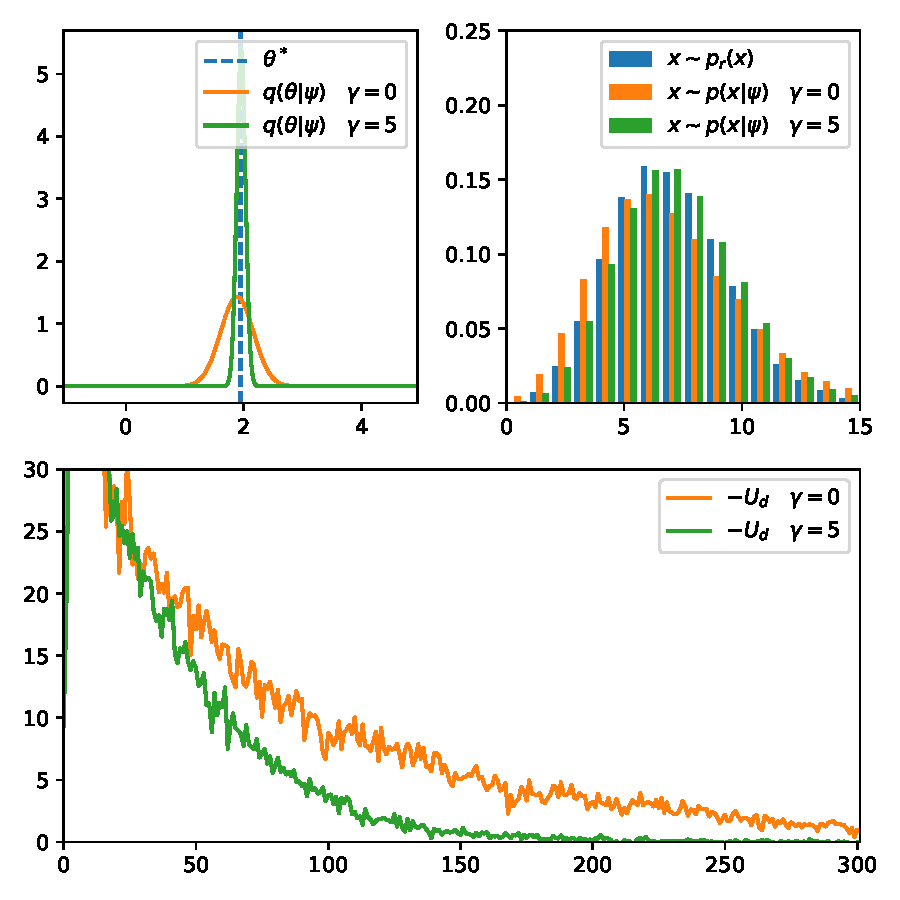
\includegraphics[width=0.48\textwidth]{figures/poisson.pdf}
    \caption{Discrete Poisson model with unknown mean.
             ({\it Top left}) Proposal distributions $q(\bftheta|\bfpsi)$ after adversarial variational optimization. For both $\gamma=0$ and $\gamma=5$, the distributions correctly concentrate their density around
                        the true value $\log(\lambda^*)$. Penalizing the entropy of the proposal distribution ($\gamma=5$) results in a tighter density.
             ({\it Top right}) Model distributions $\qxpsi$ after training. This plot shows that the resulting parameterizations of the simulator closely reproduce the true distribution.
             ({\it Bottom}) Empirical estimates of the variational upper bound $U_d$ as optimization progresses.
             }\label{fig:poisson}
\end{figure}

The top left plot in Figure~\ref{fig:poisson} illustrates the resulting proposal
distributions $q(\bftheta|\bfpsi)$ after AVO.  For
both $\gamma=0$ and $\gamma=5$, the proposal distributions correctly concentrate
their density around the true parameter value $\log(\lambda^*) = 1.94$. Under
the effect of the positive entropy penalty $H(q(\bftheta|\bfpsi))$,
the proposal distribution for $\gamma=5$ concentrates its mass more tightly,
yielding in this case a more precise inference.  The top right plot compares the
model distributions to the true distribution.  As theoretically expected from
adversarial training, we see that the resulting distributions closely match
the true distribution, with in this case visually slightly better results for the penalized
model.  The bottom plot of Figure~\ref{fig:poisson} shows empirical estimates
of $-U_d$ with respect to the epoch number. For both $\gamma=0$ and $\gamma=5$,
the curves quickly fall towards $0$, which indicates that
$\mathbb{E}_{\tilde{\mathbf{x}} \sim p(\mathbf{x}|\bftheta)}
[d(\tilde{\mathbf{x}};\phi)] \approx \mathbb{E}_{\mathbf{x} \sim
p_r(\mathbf{x})} [d(\mathbf{x};\phi)]$ and that the critic cannot distinguish
between true and model data. Despite the discreteness and the
non-differentiability of the underlying generator, this confirms that inference
with adversarial variational optimization works.


\subsection{Multidimensional continuous data}

As a second toy example, we evaluate parameter inference for a generator producing
5-dimensional continuous data, as originally specified in Section 4.2. of
\citep{cranmer2015approximating}. More specifically, we consider the following
generative process:
\begin{itemize}
    \item $\bfz = (z_0, z_1, z_2, z_3, z_4)$, such that
        $z_0 \sim {\cal N}(\mu=\alpha, \sigma=1)$,
        $z_1 \sim {\cal N}(\mu=\beta, \sigma=3)$,
        $z_2 \sim {\text{Mixture}}(\frac{1}{2}\,{\cal N}(\mu=-2, \sigma=1), \frac{1}{2}\,{\cal N}(\mu=2, \sigma=0.5))$,
        $z_3 \sim {\text{Exponential}(\lambda=3)}$, and
        $z_4 \sim {\text{Exponential}(\lambda=0.5)}$;
    \item $\mathbf{x} = R  \bfz$, where $R$ is a fixed
    semi-positive definite $5 \times 5$ matrix defining a fixed projection
    of $\bfz$ into the observed space.
\end{itemize}
We consider observed data generated at the nominal values $\bftheta^* = (\alpha^*=1,\beta^*=-1)$.
The simulator parameters are modeled with a factored Gaussian
proposal distribution $q(\bftheta|\bfpsi) = q(\alpha|\bfpsi) q(\beta|\bfpsi)$, where each component is
initialized with zero mean and unit variance.
Hyper-parameters are set to $M=64$, $n_\text{critic}=100$, $\lambda=0.025$, $\gamma=10$ and
Adam configured with $\alpha=0.01$, $\beta_1=0.9$ and $\beta_2=0.999$.
The network architecture of the critic is the same as in the previous example.

Starting with a proposal distribution $q(\bftheta|\bfpsi)$ largely spread over
the parameter space, as illustrated in the left plot of Figure~\ref{fig:multi},
inference quickly converges towards a proposal distribution whose density
concentrates around the nominal values $\bftheta^*$, as shown in the right plot of Figure~\ref{fig:multi}.
Overall, this example further illustrates and confirms the ability of adversarial
variational optimization for inference with multiple parameters and multidimensional
data, where reliable approximations of $p(\mathbf{x}|\bftheta)$ in a traditional
MLE setting would otherwise be difficult to construct.

\begin{figure}
    \centering
    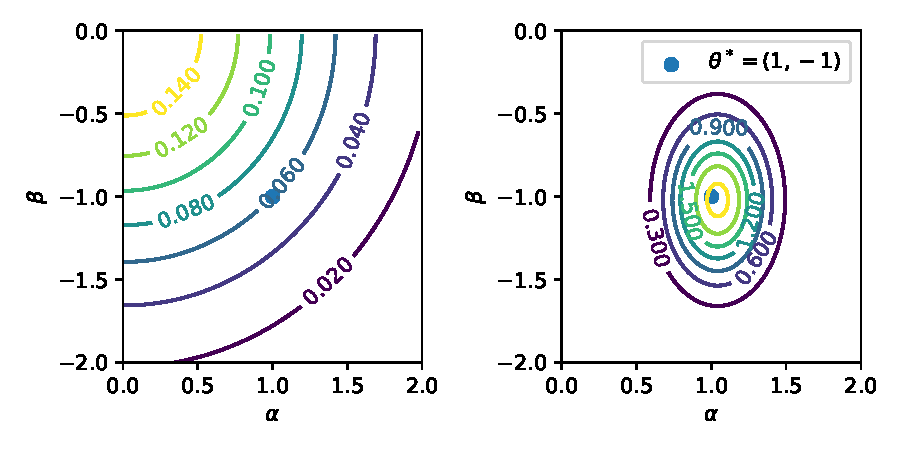
\includegraphics[width=0.48\textwidth]{figures/multi.pdf}
    \caption{Multidimensional continuous data.
             ({\it Left}) Density $q(\bftheta|\bfpsi)$ at the beginning of the procedure, for a proposal distribution initialized with zero mean and unit variance.
             ({\it Right}) Density $q(\bftheta|\bfpsi)$ after adversarial variational optimization ($\gamma=10$). The proposal density correctly converges towards a distributon whose density concentrates around $\bftheta^* = (1, -1)$.
             }\label{fig:multi}
\end{figure}


\subsection{Electron--positron annihilation}

As a more challenging example, we now consider a (simplified) simulator from
particle physics for electron--positron collisions resulting in muon--antimuon
pairs ($e^+e^- \rightarrow \mu^+\mu^-$). The simulator approximates the
distribution of observed measurements $\mathbf{x} = \cos(A) \in [-1,1]$, where $A$ is the
polar angle of the outgoing muon with respect  to the originally incoming
electron. This random variable is approximately distributed as
\begin{equation}
    p(\mathbf{x}|E_\text{beam}, G_f) = \frac{1}{Z} \left[ (1 + \mathbf{x}^2) + c(E_\text{beam}, G_f) \mathbf{x} \right]
\end{equation}
where $Z$ is a known normalization constant and $c$ is an asymmetry coefficient
function. Due to the linear term in the expression, the density $p(\mathbf{x} |
E_\text{beam}, G_f)$ exhibits a so-called {\it forward-backward} asymmetry.  Its
size depends on the values of the parameters $E_\text{beam}$ (the beam energy)
and $G_f$ (the Fermi constant) through the coefficient function $c$. Given the
known analytic form of the probability density function, a simulator for
$\mathbf{x}$ can be implemented with rejection sampling~\citep{von195113}. As an
arbitrary number of random drawings may be required before passing the
acceptance threshold, this illustrates how the latent variable
$\bfz$ does not necessarily need to be fixed-sized vector, and how its
density  $p(\bfz|\bftheta)$ may depend on $\bftheta$ in some complicated way
(Section~\ref{sec:problem}).

In this example, we consider observed data generated with $\bftheta^* =
(E_\text{beam}^*=42, G_f^*=0.9)$. The simulator parameters are modeled with a
factored Gaussian proposal distribution $q(\bftheta|\bfpsi) = q(E_\text{beam}|\bfpsi)
q(G_f|\bfpsi)$, where each component is respectively initialized with mean $45$
and $1$ and variance $1$ and $0.01$. Hyper-parameters are set to $M=64$,
$n_\text{critic}=100$, $\lambda=0.0025$ and Adam configured with $\alpha=0.01$,
$\beta_1=0.9$ and $\beta_2=0.999$. As for the first example, we compare
entropy penalties $\gamma=0$ and $\gamma=5$.

The top left plot in Figure~\ref{fig:weinberg} illustrates the resulting
proposal distributions $q(\bftheta|\bfpsi)$ for $\gamma=0$ and $\gamma=5$ after
AVO. We see that the distributions both arrive
in the neighborhood of $\bftheta^*$, with a density  more highly concentrated for
$\gamma=5$ than for $\gamma=0$.  Despite these differences and the relative
distance with $\bftheta^*$, both models closely match the observed data, as shown
in the top right plot of  Figure~\ref{fig:weinberg}, with again slightly better
results for the entropy penalized model. This suggests either a relatively flat
landscape around $\bftheta^*$ or that the observed data can in this case also be
reproduced with a smeared variation $\qxpsi$ of the simulator.
Finally, the bottom plot of Figure~\ref{fig:weinberg} shows that for both
$\gamma=0$ and $\gamma=5$ the variational upper bound $-U_d$ quickly fall
towards $0$, which indicates  convergence towards a distribution that the critic
cannot distinguish from the true distribution. In summary, despite the intricate
relation betwen the observations $\mathbf{x}$, the latent variable $\bfz$
and the parameters $\bftheta$, this example demonstrates the efficacy
of AVO for parameter inference on a black box
simulator.

\begin{figure}
    \centering
    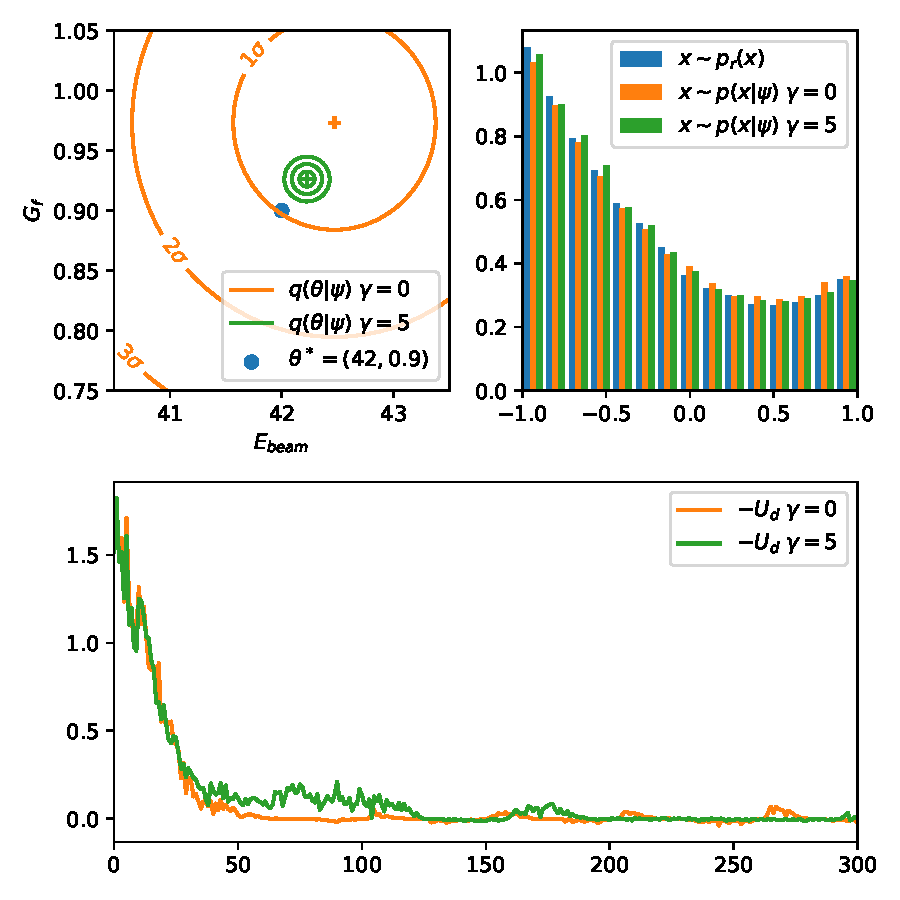
\includegraphics[width=0.48\textwidth]{figures/weinberg.pdf}
    \caption{Electron--positron annihilation.
    ({\it Top left}) Proposal distributions $q(\bftheta|\bfpsi)$ after adversarial variational optimization. The density of the penalized distribution ($\gamma=5$) is here highly concentrated, resulting in the green mass near $\bftheta^*$.
    ({\it Top right}) Model distributions $\qxpsi$ after training. Despite the differences between their respective proposal distributions, both models closely match the observed data.
    ({\it Bottom}) Empirical estimates of the variational upper bound $U_d$ as optimization progresses.
             }\label{fig:weinberg}
\end{figure}


% ==============================================================================

\section{Related works}

As reviewed in \cite{2016arXiv161003483M}, likelihood-free inference is
intimately tied to a class of algorithms that can be framed as density
estimation-by-comparison. In most cases, these inference algorithms are
formulated as an iterative two-step process where the model distribution is
first compared to the true data distribution and then updated to make it more
comparable to the latter.

Closest to our work are procedures that rely on a classifier to estimate the
discrepancy between the true and the model distributions. For example,
\citep{gutmann2012noise} uses non linear logistic regression for fitting
unnormalized differentiable statistical models, while
\citep{goodfellow2014generative} exploits an adversarial neural network for
learning a differentiable implicit generative model. In the likelihood-free
setup, \citep{cranmer2015approximating,cranmer2016experiments,2016arXiv161110242D} estimate likelihood
ratios through supervised classification, which can in turn be used for
parameter inference in combination with a gradient-free optimization algorithm.
Similarly, \citep{gutmann2017likelihood} makes use of classification accuracy as
a summary statistics for approximate Bayesian computation.

In this context, the proposed method can be considered as a direct adaptation of
generative adversarial networks~\citep{goodfellow2014generative} to
non-differentiable simulators. It also constitutes an approximate gradient
descent alternative to likelihood-free inference based on bayesian optimization and approximated density
ratios~\citep{cranmer2015approximating,cranmer2016experiments} or to classifier
ABC~\citep{gutmann2017likelihood}.

This work has many connections to variational inference, in which the goal is to optimize the recognition model $q(\bftheta|\bfpsi)$ so that it is close to the true posterior $p(\bftheta|x)$. This is slighty different from variational optimization (or variational learning), where the toal is to find $\bftheta^*$ such that $p(x|\bftheta^*) \approx p_r(x)$.  Typically in variational inference the model $p(x|\bftheta)$ admits a density, so that the likelihood is known. Thus, assuming the prior also admits a density, it is tractable to evaluate the posterior is (up to a constant factor). In Adversarial Variational Bayes \citep{DBLP:journals/corr/MeschederNG17} and , equivalently, the \texttt{PC-Adv} algorithm of  \citep{2017arXiv170208235H}), the authors use an adversarial setup, but assume a known density $p(x|\bftheta)$ that is differentiable with respect to $\bftheta$. 

In \citep{tran2017variational}, the authors consider Variational Bayes with an intractable likelihood. In that approach "The only requirement is that the intractable likelihood can be estimated unbiasedly.'' In the case of most simulators it is not clear how one would obtain the unbiased estimator $\hat{p}(x|\bftheta)$.


In \citep{2017arXiv170208235H} the author defines implicit distributions to be ``probability models whose probability density function may be intractable, but there is a way to 1) sample from them exactly and/or calculate and approximate expectations under them, and 2) calculate or estimate gradients of such expectations with respect to model parameters.'' This notion of implicit model does not include most scientific simulators as 2) is not satisfied. The  \texttt{JC-Adv} and \texttt{JC-Den} algorithm defined there applies to implicit models, but, as the author points out, is aimed at variational inference and ``does not provide a direct way to learn model parameters $\bftheta$''.



% ==============================================================================

\section{Summary}

In this note, we develop a likelihood-free inference algorithm for fitting a
forward non-differentiable simulator to continuous or discrete observed data.
The algorithm combines adversarial training  with variational optimization to
minimize variational upper bounds  on the otherwise non-differentiable
adversarial objectives.
Effectively, the procedure results in learning an arbitrarily tight proposal
distribution over the simulator parameters, such that corresponding the marginal
distribution of the generated data matches the observations. Preliminary results
with non-differentiable discrete or continuous simulators validate the proposed method.

While the obtained results are encouraging, the complete validation of the
method remains to be carried out in real conditions on a full fledged scientific
simulator -- which we plan to achieve for a next version of this work.
In terms of method, several components need to be further investigated.
First, we need to better study the interplay between the entropy penalty and the adversarial objectives.
Second, we should better understand the dynamics of the optimization
procedure, in particular when combined with momentum-based optimizers like Adam.
Third, we need to consider whether less noisy estimates of the gradients
$\nabla_\bfpsi U_g$ can be computed, in particular by exploiting the fact in the composition $d(g(\bfz;\bftheta); \bfpsi)$
the derivatives of $d$ are known exactly.


\textbf{KC: could also use this to tune non-differentialble fast simulator to slower full simulator. Then fixed data size not an issue}

% ==============================================================================

\section*{Acknowledgments}

We would like to thank Lukas Heinrich for helpful comments regarding
the electron--positron annihilation simulation.

GL and KL are both supported through NSF ACI-1450310, additionally KC is
supported through PHY-1505463 and PHY-1205376.


% ==============================================================================

\bibliographystyle{acm}
\bibliography{bibliography.bib}

\end{document}
